\renewcommand{\lstlistingname}{kódrészlet}

\chapter{A felismerő megvalósítása}
\section{Alkalmazott módszerek}
A felismerő program megvalósítása során az eddig megismert módszereket fogom felhasználni, azokat C++ programozási nyelven fogom elkészíteni és ismertetni. Az egyes algoritmusokat függvények formájában készítem el, ezeket a függvényeket pedig több helyen is felhasználom.
\par Az eddig megismert módszerek közül elsősorban a nyers bemenetből emelem ki a játékterületet, ezt követően a golyók pozíciójának felismeréséhez kör detektálást és egy neurális hálózatot fogok használni. A következőkben az egyes függvények működését, azokban felhasznált külső könyvtárak eszközeit ismertetem részleteiben.
\par A fejezetek felosztása az eddig megismert lépések szerint kerül rendezésre.

\section{A szükséges könyvtárak importálása}
Ahhoz hogy a függvények megfeleően működjenek, meg kell mondani a programnak, hogy használja a külső könyvtárakat.
\newline A legfontosabb könyvtárak importálása a \ref{cod:import} kódsorok alapján tehető meg.

\vspace{2mm}
\hspace{-10mm}
\begin{minipage}{\linewidth}
\begin{lstlisting}[language=C++, numbers=left, caption={Könyvtárak importálása.}, label={cod:import}]
#include <opencv2/opencv.hpp>
#include <fdeep/fdeep.hpp>
\end{lstlisting}
\end{minipage}

\par Az \lstinline{opencv.hpp} könyvtár az OpenCV által biztosított képfeldolgozási függvényeket biztosítja, a \lstinline{fdeep.hpp} könyvtár pedig a Tensorflow -al készített neurális hálózat betöltését teszi lehetővé.

\section{Az asztal kontúrjának megkeresése}
\label{section:megv_asztal_kontur}
A nyers képből a játékterület megszerzéséhez azt először be kell tölteni egy többdimenziós tömbbe. A kép betöltése többféleképp végbemehet, ezért ezt konkrétan nem részletezem.
\par A betöltött kép tömbjének alakja megegyezik a kép szélességével és magasságával, továbbá az intenzitási értékekkel, tehát egy 1024 x 512 méretű RGB képet betöltve, annak tömbjének az első és második dimenziója 1024 és 512, a harmadik pedig az RGB (Piros, Zöld, Kék) intenzitásoknak megfelelően 3 méretű.
\par Fontos megjegyezni, hogy az OpenCV a képeket betöltéskor BGR formátumban tölti be, ez az elnevezésből adódóan annyiban tér el az RGB formátumtól, hogy a piros (R) és kék (B) színcsatornák fel vannak cserélve.
\par A nyers bemeneti kép megszerzése után következik az asztal kontúrjának megkeresése. Első lépésként a képet HSV formátumra kell alakítani, majd az alsó és felső intenzitási értékhatárok megadásával meghatározható a maszk, amely alkalmazható az eredeti képre.
\newline A fentieket a \ref{cod:maszk} kódrészlettel végzem el.


\vspace{2mm}
\hspace{-10mm}
\begin{minipage}{\linewidth}
\begin{lstlisting}[language=C++, numbers=left, caption={A játékterület maszkolása.}, label={cod:maszk}]
cv::cvtColor(image, hsv, cv::COLOR_BGR2HSV);

cv::Scalar lowerGreen = {50, 50, 70};
cv::Scalar upperGreen = {65, 255, 255j};

cv::inRange(hsv, lowerGreen, upperGreen, mask);
cv::bitwise_and(image, image, result, mask);
\end{lstlisting}
\end{minipage}

\par A \ref{cod:maszk} kódrészletben az \lstinline{image} a bemeneti kép, amelyet a \lstinline{cv::cvtColor} függvénnyel \cite{opencv_docs} konvertálok át HSV formátumra. Ennek a függvénynek az első paramétere a bemeneti kép, a második a kimeneti kép változója, a harmadik pedig a konverzió típusa, amely ebben az esetben BGR $\rightarrow$ HSV.
\par A BGR értékekből a HSV értékek kiszámolásához először az értéket (Value) kell kiszámolni, ez a \ref{for:HSV_V} egyenlet\cite{opencv_docs} szerint lehetséges,

\begin{equation}
    V \leftarrow max(R,G,B)
    \label{for:HSV_V}
\end{equation}

\par ahol $V$ az értéket (Value) jelöli, $R$, $G$ és $B$ pedig az adott képpont három színkomponensét (Piros, Zöld, Kék). Az egyenlet alapján az érték a három színkomponens közül a legnagyobbnak az értékét fogja felvenni. Az érték kiszámolásával megadható a telítettség (Saturation).
\par Ezt a \ref{for:HSV_S} egyenlet\cite{opencv_docs} alapján lehet kiszámolni,

\begin{equation}
    S \leftarrow
    \begin{cases}
        \frac{V-min(R,G,B)}{V} & ,\text{ha}\ V\neq0 \\
        0 & ,\text{különben}
    \end{cases}
    \label{for:HSV_S}
\end{equation}

\par itt $S$ a telítettséget (Saturation) jelöli, és az előzőekhez hasonlóan $V$ az értéket (Value), $R$, $G$ és $B$ pedig a színkomponenseket, továbbá $min(R,G,B)$ a három színkomponens közül a legkisebbet adja meg.
\par Az árnyalatot (Hue) szintén az érték (Value) segítségével lehet kiszámolni, ezt a \ref{for:HSV_H} egyenlet\cite{opencv_docs} adja meg,

\begin{equation}
    H \leftarrow
    \begin{cases}
        \frac{60(G-B)}{V-min(R,G,B)} & ,\text{ha}\ V=R \\[5pt]
        \frac{120+60(B-R)}{V-min(R,G,B)} & ,\text{ha}\ V=G \\[5pt]
        \frac{240+60(R-G)}{V-min(R,G,B)} & ,\text{ha}\ V=B \\[5pt]
        0 & ,\text{ha}\ R=G=B
    \end{cases}
    \label{for:HSV_H}
\end{equation}

\par ahol $H$ az árnyalatot (Hue), $V$ az értéket (Value), $R$, $G$ és $B$ a három színkomponenst, $min(R,G,B)$ pedig a színkomponensek közül a minimálisat jelöli.
\par Amennyiben $H$ értéke kisebb, mint $0$, annak értéke $H \leftarrow H+360$ szerint alakul. A 8-bites és 16-bites színnel rendelkező képeknél $R$, $G$ és $B$ értéke kezdetben normalizálásra kerül a $[0,1]$ intervallumba, ennek következtében a három értéknél $0 \le V \le 1$, $0 \le S \le 1$, $0 \le H \le 360$ tartományok jelentkeznek. Az értékek visszaállítása tartománynak megfelelően 8-bites képek esetében az értékek megszerzése után $V \leftarrow 255V$, $S \leftarrow 255S$ és $H \leftarrow H/2$ szerint megy végbe, ez hasonló 16-bites szín esetében is. 32-bites színnel rendelkező képeknél nincs kezdeti normalizálás, és ennek következtében visszaalakítás sem szükséges.\cite{opencv_docs}

\par Az \ref{cod:maszk} kódrészlethez visszatérve, a \lstinline{lowerGreen} és \lstinline{upperGreen} változók az alsó és felső intenzitási határokat jelölik sorrendnek megfelelően. A maszk elkészítését a \lstinline{cv::inRange} függvénnyel \cite{opencv_docs} végzem el, itt a paraméterek sorban a HSV re konvertált kép, az alsó és felső intenzitás értékek, valamint a kimeneti maszk változója.
\newline A függvény a \ref{for:maszkolas} egyenlet alapján dönti el, a maszk intenzitását,

\begin{equation}
    M(I) = L(I) \le S(I) \le U(I)
    \label{for:maszkolas}
\end{equation}

\par ahol $M$ a maszk, $L$ az alsó, $U$ a felső és $S$ a bemeneti HSV képet jelöli. A \ref{for:maszkolas} függvény mindhárom intenzitásra alkalmazásra kerül, a maszkban az intervallumon belüli intenzitások 255, a kívüliek pedig 0 értéket kapnak. A maszk elkészítése után a maszkolás megtörténik az eredeti bemenő képre a \lstinline{cv::bitwise_and} függvény \cite{opencv_docs} segítségével. Itt a paraméterek a bejövő eredeti kép \lstinline{image} kétszer, a kimeneti kép és a maszk \lstinline{mask}.
\newline A folyamat során a metódus a \ref{for:maszk_alkalmazas} egyenlet szerint jár el,

\begin{equation}
    R(I) = S_1(I)\quad \land\quad S_2(I)\qquad ,ha\quad M(I) \ne 0
    \label{for:maszk_alkalmazas}
\end{equation}

\par ahol $R$ a kimenő maszkolt kép (\lstinline{result}) $S_1$ és $S_2$ a két bemeneti kép paraméter, és $M$ a maszk. A bemenetben a kép azért szerepel kétszer egymás után, mert a \ref{for:maszk_alkalmazas} függvényben láthatóan a két bemenő paraméter közt egy bit szintű 'és' művelet történik, amennyiben a maszk nem nulla. Ennek eredményeképp az eredeti kép adódik vissza amelyen maszkolt képpontok feketével szerepelnek. Ez azért történik, mert bit szinten ha két megegyező elem közt történik 'és' művelet, akkor az eredmény szintén megegyezik a két elemmel. Ennek a folyamatnak a kimenetele látható a már előzőleg tárgyalt \ref{fig:bemeneti_kep_mask} ábrán.
\par A maszkolt kép megszerzése után elvégezhető az éldetektálás, amelyet megelőz egy szürkeárnyalatolás.

\vspace{2mm}
\hspace{-10mm}
\begin{minipage}{\linewidth}
\begin{lstlisting}[language=C++, numbers=left, caption={Szürkeárnyalatolás és éldetektálás.}, label={cod:gray_and_canny}]
cv::cvtColor(result, imageGray, cv::COLOR_BGR2GRAY);

cv::Canny(imageGray, edges, 200, 100);
\end{lstlisting}
\end{minipage}

\par A szürkeárnyalati konverziót a már megismert \lstinline{cv::cvtColor} függvénnyel \cite{opencv_docs} végzem el a \ref{cod:gray_and_canny} kódrészlet alapján, majd ezután megkeressem az éleket a képen Canny éldetektálás \cite{opencv_docs, canny_edge_detection} (\lstinline{cv::Canny}) segítségével.
\newline A Canny éldetektálás általában több lépésre bontható szét, ezek lehetnek:

\begin{itemize}
    \setlength\itemsep{-2pt}
    \item homályosítás Gauss szűrővel \cite{shapiro2001} a zajcsökkentés érdekében,
    \item élek helyének és irányának megállapítása intenzitás-gradiensből,
    \item nem-maximum vágás merőleges élek szűréshéhez,
    \item kettős küszöbölés élek szűréséhez.
\end{itemize}

\par Az éldetektálásnál meg kell adni a függvénynek a szürkeárnyalatos képet (\lstinline{imageGray}), a kimeneti képet, továbbá két küszöbértéket, amelyet a Canny detektálás a kettős küszöbölés folyamat során fog felhasználni. Itt, ha a felső küszöb felett van egy potenciális él, az hozzáadódik az élek közé, ha az alsó küszöb alatt van eldobódik és ha a felső és alsó küszöbök közt helyezkedik el, akkor a szomszédos pixelek alapján kerül az élek közé. Az éldetektálással kapott kép (\lstinline{edges}) a \ref{fig:bemeneti_kep_edge} ábrán látható.

\begin{figure}[!ht]
    \centering
    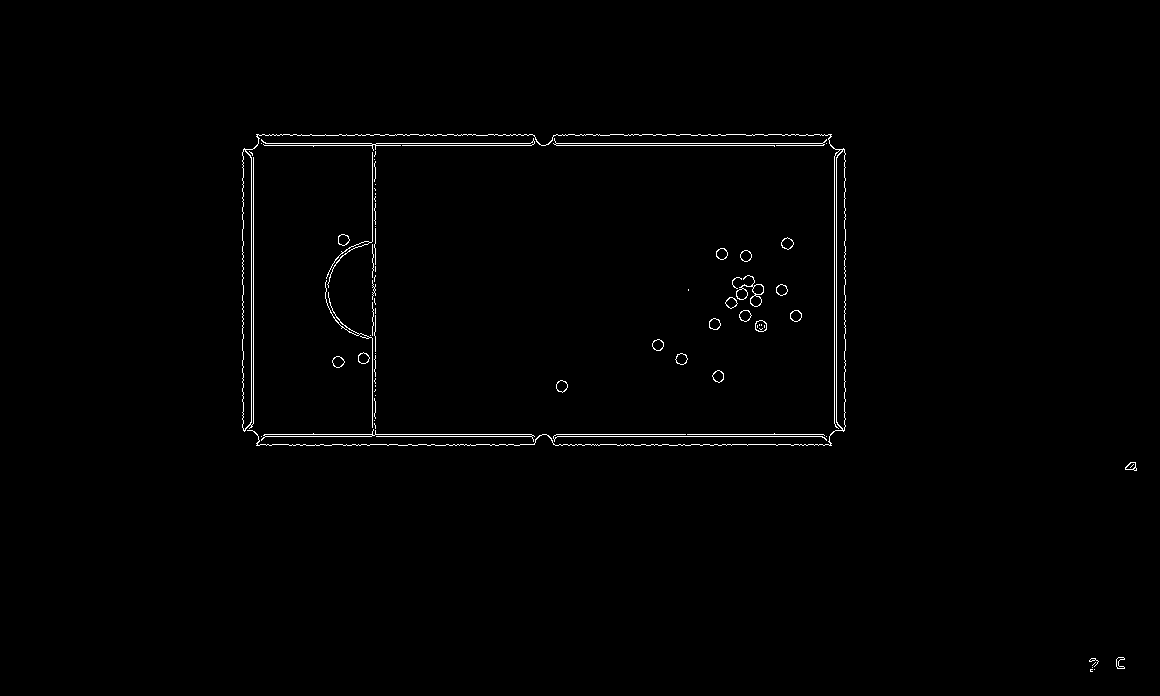
\includegraphics[width=140mm, keepaspectratio]{figures/input_screen_edge.png}
    \caption{A Canny éldetektálás után kapott kép.}
    \label{fig:bemeneti_kep_edge}
\end{figure}

\par A következő lépésben a bináris képen lefuttatásra kerül egy kontúrkereső algoritmus \cite{SUZUKI198532}, majd a kapott kontúroknak vesszem a konvex körvonalát, azok egyszerűsítése, esetleges konkáv alakzatok megszüntetése érdekében. Ezek után feltételezve, hogy a kontúrok közül a legnagyobb a játékterület, az kiválasztható a körvonalak közül.

\vspace{2mm}
\hspace{-10mm}
\begin{minipage}{\linewidth}
\begin{lstlisting}[language=C++, numbers=left, caption={Kontúrok keresése.}, label={cod:contours}]
cv::findContours(edges, contours, cv::RETR_LIST, cv::CHAIN_APPROX_SIMPLE);

for(auto& contour : contours) {
    std::vector<cv::Point> hull;
    cv::convexHull(contour, hull);
    contour = hull;
}

std::sort(contours.begin(), contours.end(), areaComparator);
\end{lstlisting}
\end{minipage}

\vspace{2mm}
\hspace{-10mm}
\begin{minipage}{\linewidth}
\begin{lstlisting}[language=C++, numbers=left, caption={Sorba rendezéshez használt segédfüggvény.}, label={cod:contours_helper}]
bool areaComparator(const std::vector<cv::Point>& lhs, const std::vector<cv::Point>& rhs) {
    return cv::contourArea(lhs) > cv::contourArea(rhs);
}
\end{lstlisting}
\end{minipage}

\par A \ref{cod:contours} kódrészletben található \lstinline{cv::findContours} függvény \cite{opencv_docs, SUZUKI198532} egy határkövetéses algoritmussal kigyűjti a kontúrokat. Ezek a kontúrok a képen található képpont koordináták láncolatából állnak össze. A kontúrok körvonala a \lstinline{cv::convexHull} függvény \cite{opencv_docs, SKLANSKY198279} segítségével kapható meg. Ez az algoritmus a kontúrok koordinátáinak láncolatát használja, majd a kontúrt egy konvex körvonallal határolja, ugyancsak koordináták láncolatai formájában reprezentálva.
\par A fenti művelet elsőre feleslegesnek tűnhet, hiszen a keresett asztal kontúrja előreláthatólag nem konkáv, a művelet elvégzése mégis fontos, hiszen így egyszerűsíthető az alakzat (kontúr koordináta láncolat pontjainak csökkentése), ezzel a folytatólagos műveleteket felgyorsítva.
\par A legnagyobb kontúr kiválasztásához tudni kell az egyes kontúrok területét. A területet a \lstinline{cv::contourArea} függvénnyel \cite{opencv_docs} lehet kiszámolni. Ez megtehető minden eddigi kontúr esetében függvénynek való paraméterkénti átadással. A kiszámolt területek közül a legnagyobbat kiválasztva, annak kontúr koordináta láncolata eltárolásra kerül. A sorba rendezés a \ref{cod:contours} kódrészlet utolsó sorában látható függvénnyel történik, itt az \lstinline{areaComparator} egy segédfüggvény, amely az előzőleg említett \lstinline{cv::contourArea} metódust\cite{opencv_docs} használja a területek összehasonlításához és rendezéséhez. A segédfüggvény a \ref{cod:contours_helper} kódrészletben látható. A kapott kontúr kirajzolva a \ref{fig:bemeneti_kep_contour} ábrán látható.

\begin{figure}[!ht]
    \centering
    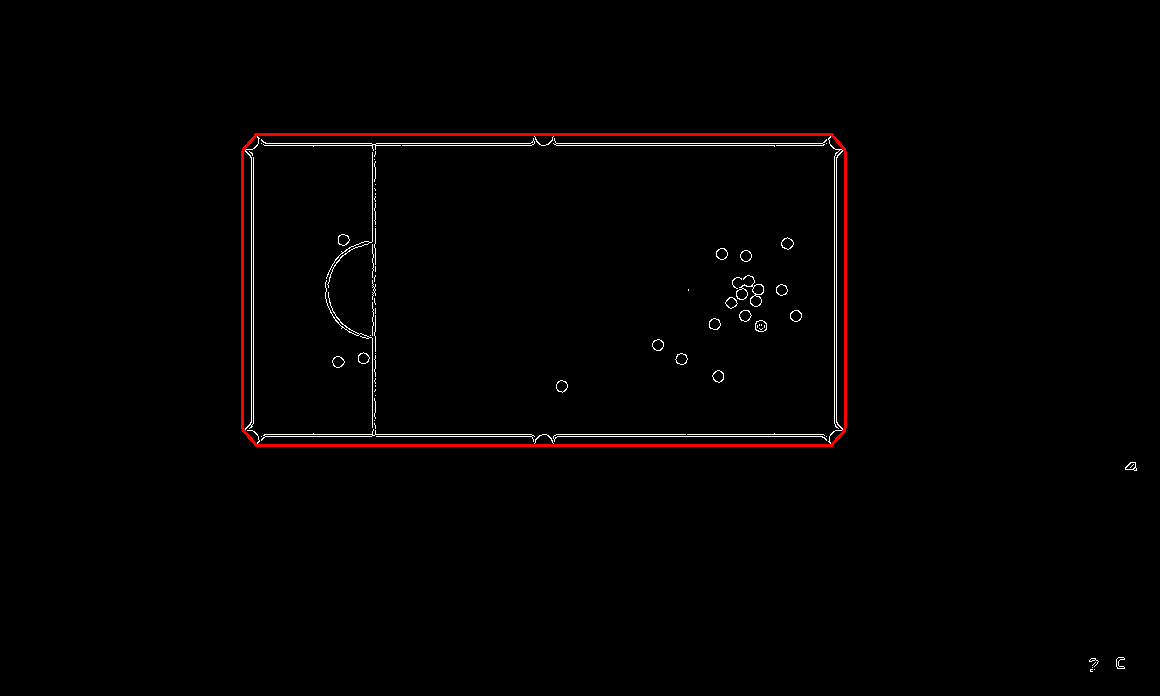
\includegraphics[width=140mm, keepaspectratio]{figures/input_screen_contour.png}
    \caption{A felismert asztal kontúrja a bináris képen, piros körvonallal keretezve.}
    \label{fig:bemeneti_kep_contour}
\end{figure}

\par A \lstinline{cv::contourArea} függvény a Surveyor's Area algoritmust \cite{braden1986surveyor} használja az alakzatok területének számolásához. Ez az algoritmus a Green-tétel egy speciális esete, amely alkalmazható egyszerű sokszögekre.
\newline Az algoritmus a \ref{for:green_formula} egyenletben látható,

\begin{equation}
    A = \sum^n_{k=0}\frac{(x_{k+1} + x_k)(y_{k+1} - y_k)}{2}
    \label{for:green_formula}
\end{equation}

\par ahol $n$ az óramutató járásával ellentétesen rendezett kontúr koordináták száma, $(x_k, y_k)$ a $k$ adik koordináta $x$ és $y$ pozíciója, és feltételezhető, hogy a $k = n+1$ elem megegyezik a $k = 0$ elemmel.

\par A \ref{fig:bemeneti_kep_contour} ábrán látható, hogy a kontúr téglalaphoz hasonló alajkának ellenére több, mint 4 pontból áll. Ahhoz hogy téglalap formájában legyen kivágva a kép, meg kell keresni azt a négyszöget, amely a kontúrt határolja. Erre egy olyan algoritmust készítettem, amely megkeresi a kontúr koordináták segítségével a négy leghosszabb oldalt, majd kiszámolja ezek metszéspontját. A négy leghosszabb oldal használata feltételezi, hogy a kép közel felső nézetből készült az asztalró, továbbá, hogy a sarkoknál jelenik meg több pont a kontúr keresés után.
\par Az oldalhosszok számolása a \ref{for:vector_distance} képlet alapján megy végbe,

\begin{equation}
    D = \sqrt{(x_a-x_b)^2 + (y_a-y_b)^2}
    \label{for:vector_distance}
\end{equation}

\par ahol $D$ a kiszámolt pontok közti távolság, $(x_a,y_a)$ és $(x_b,y_b)$ pedig a két koordináta, ameyek közt a táv számolandó. Miután megvannak az oldalak hosszai, eltárolásra kerül a négy legnagyobb oldalhoz tartozó koordináta. A kiválasztott pontoknál fontos, hogy óramutató járásával ellentétes sorrendben legyenek rendezve, amennyiben nem, a négyszög kontúr később hibás lehet.
\par A metszéspontok kiszámolásához a következő képleteket \cite{line_line} használtam,

\begin{equation}
    D = (x_1 - x_2)(y_3 - y_4) - (y_1 - y_2)(x_3 - x_4)
    \label{for:vector_intersection_denominator}
\end{equation}
\begin{equation}
    P_x = \frac{(x_1y_2 - y_1x_2)(x_3 - x_4) - (x_3y_4 - y_3x_4)(x_1 - x_2)}{D}
    \label{for:vector_intersection_point_x}
\end{equation}
\begin{equation}
    P_y = \frac{(x_1y_2 - y_1x_2)(y_3 - y_4) - (x_3y_4 - y_3x_4)(y_1 - y_2)}{D}
    \label{for:vector_intersection_point_y}
\end{equation}

\par ahol a \ref{for:vector_intersection_denominator} képletben a $D$ a \ref{for:vector_intersection_point_x} és \ref{for:vector_intersection_point_y} képletekben a nevező kiszámolásához biztosít könnyebb átláthatóságot, $(P_x, P_y)$ a kiszámolt metszéspont, $(x_1, y_1)$, $(x_2, y_2)$, $(x_3, y_3)$ és $(x_4, y_4)$ pedig a négy pont, amelyek a két egyenest határozzák meg, itt ezek közül az első kettő az egyik, a második kettő a másik egyeneshez tartozik.
\par A fenti egyenletek megvalósítása a \ref{cod:intersection} kódrészletben látható,

\vspace{2mm}
\hspace{-10mm}
\begin{minipage}{\linewidth}
\begin{lstlisting}[language=C++, numbers=left, caption={Metszéspont kereső algoritmus.}, label={cod:intersection}]
bool parallel = false;
cv::Point p1, p2, p3, p4, intersection;
float d, t1, t2;

d = (p1.x - p2.x) * (p3.y - p4.y) - (p1.y - p2.y) * (p3.x - p4.x);

if (std::abs(d) < 1e-8) {
    parallel = true;
}

if (!parallel) {
    t1 = (p1.x*p2.y - p1.y*p2.x) * (p3.x - p4.x) - (p3.x*p4.y - p3.y*p4.x) * (p1.x - p2.x);
    t2 = (p1.x*p2.y - p1.y*p2.x) * (p3.y - p4.y) - (p3.x*p4.y - p3.y*p4.x) * (p1.y - p2.y);
    
    intersection = cv::Point(t1 / d, t2 / d);
}
\end{lstlisting}
\end{minipage}

\par ahol \lstinline{p1}, \lstinline{p2}, \lstinline{p3}, \lstinline{p4} a fent megismert négy koordináta, \lstinline{d} a kiszámolt nevező, \lstinline{t1} és \lstinline{t2} pedig segédváltozók a számlálók tárolásához. A kódrészlet 7. - 9. soraiban látható, hogy abban az esetben ha \lstinline{d} nagyon kicsi, a metszéspont nem lesz kiszámolva. Ez azért van, mert a \ref{for:vector_intersection_denominator} függvényben kiszámolt nevező, $D = 0$ esetén a két egyenes párhuzamos, és ilyenkor nincs metszéspont.
\par A folyamat végeredményeképp kapott kép a \ref{fig:bemeneti_kep_quad} ábrán látható.

\begin{figure}[!ht]
    \centering
    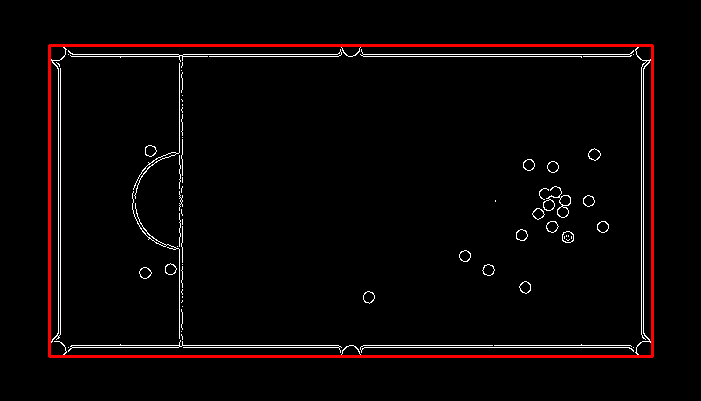
\includegraphics[width=140mm, keepaspectratio]{figures/input_screen_quad.png}
    \caption{A felismert asztal négy pontból álló körvonala a bináris képen, piros körvonallal keretezve.}
    \label{fig:bemeneti_kep_quad}
\end{figure}

\section{Az asztal kivágása és torzítása}
Ahhoz, hogy az asztal a kontúr segítségével kivágható legyen a képből, szükség lesz egy téglalapra, amely alapján a kivágás elvégezhető. Ebben a részben ennek a folyamatnak a működéséről fogok beszélni.
\par A folyamat első részeként a kapott, négy koordinátából álló kontúr pontjait rendezni kell. A pontokat bal felső, jobb felső, jobb alsó és bal alsó pontok szerint kell sorba rendezni.
\newline Az átrendezéshez a \ref{cod:atrendezes} kódot használom,

\vspace{2mm}
\hspace{-10mm}
\begin{minipage}{\linewidth}
\begin{lstlisting}[language=C++, numbers=left, caption={Átrendező algoritmus.}, label={cod:atrendezes}]
std::vector<int> sums, diffs;

for (auto& point : quad) {
    sums.push_back(point.x + point.y);
    diffs.push_back(point.y - point.x);
}

std::vector<cv::Point2f> src;
src.push_back(quad[std::min_element(sums.begin(), sums.end()) - sums.begin()]);
src.push_back(quad[std::min_element(diffs.begin(), diffs.end()) - diffs.begin()]);
src.push_back(quad[std::max_element(sums.begin(), sums.end()) - sums.begin()]);
src.push_back(quad[std::max_element(diffs.begin(), diffs.end()) - diffs.begin()]);
\end{lstlisting}
\end{minipage}

\par ahol az előzőleg kiszámolt négy metszéspontot felhasználva, ahhoz hogy meg tudjam állapítani a azok relatív helyzetét, készítek az egyes pontokból összegeket (\lstinline{sums}) és különbségeket (\lstinline{diffs}), amelyek az egyes koordináták $x$ és $y$ összetevőinek összegeiből vagy különbségeiből állnak. Ezekből az összegek és különbségekből megállapítható a pontok helyzete, tehát például a bal felső koordinátát az összegek közül a legkisebb érték, a bal alsót a különbségek közül a legnagyobb érték határozza meg, és így a többi koordinátát is. A fent említett műveletek a kódrészlet 9. - 11. soraiban láthatóak.
\par Az előző művelet után a sorba rendezett koordináták meghatározzák a transzformációhoz szükséges mátrix kiszámításához a forrás (\lstinline{src}) értékeket. A transzformációhoz szükség van még a célértékekre is.
\newline A célértékek a \ref{cod:destination} kód soraival adhatóak meg,

\vspace{2mm}
\hspace{-10mm}
\begin{minipage}{\linewidth}
\begin{lstlisting}[language=C++, numbers=left, caption={A kimeneti értékek megadása.}, label={cod:destination}]
std::vector<cv::Point2f> dst;

int width = 1024 - 1;
int height = 512 - 1;

dst.push_back(cv::Point(0, 0));
dst.push_back(cv::Point(width, 0));
dst.push_back(cv::Point(width, height));
dst.push_back(cv::Point(0, height));
\end{lstlisting}
\end{minipage}

\par itt a cél kép méretei egy érték páros formájában szerepelnek a \lstinline{width} és \lstinline{height} változókban. Az értékekből egyet való levonás az indexelés végett szükséges. A szélesség és magasság értékekkel ezután meg lehet adni a célértékeket a transzformációs mátrix elkészítéséhez, ezek a \lstinline{dst} változóba kerülnek.
\par A transzformáció végrehajtásához mindezek után már csak a transzformációs mátrix elkészítésére van szükség, majd a transzformáció végrehajtására.
\newline Ezek a \ref{cod:pers_transform} kódrészlettel hajthatóak végre,

\vspace{2mm}
\hspace{-10mm}
\begin{minipage}{\linewidth}
\begin{lstlisting}[language=C++, numbers=left, caption={A transzformáció végrehajtása.}, label={cod:pers_transform}]
cv::Mat M = cv::getPerspectiveTransform(src, dst);
cv::warpPerspective(image, warp, M, cv::Size(width, height));
\end{lstlisting}
\end{minipage}

\par itt \lstinline{M} a transzformációs mátrix, amely a \lstinline{cv::getPerspectiveTransform} függvénnyel \cite{opencv_docs} kapható meg a forrás és célértékek megadásával. A függvény Gauss-elimináció \cite{grcar2011mathematicians} segítségével számol ki egy $3\times3$ méretű mátrixot, amelyet a \lstinline{cv::warpPerspective} függvénnyel \cite{opencv_docs} alkalmazok az \lstinline{image} változóban tárolt képre az \lstinline{M} mátrix és \lstinline{cv::Size(width, height)} méret megadásával. A transzformáló függvény lineáris interpolációt \cite{blu0401interpolation} használ alapértelmezett esetben az intenzitás értékek meghatározásához, a torzított kép a \lstinline{warp} változóban kerül tárolásra.
\par A kivágott és torzított kép a már megismert \ref{fig:bemeneti_asztal2} ábrán látható.

\section{Körkeresés}
A körök detektálásához az ún. Hough transzformációt (Hough Transformation) fogom használni, ez a H.K. Yuen, J. Princen, J. Illingworth és J. Kittler et. al. 1990 \cite{YUEN199071} szerint abban az esetben, ha egy kör a kövekező \ref{for:hough_transform} függvénnyel írható le,

\begin{equation}
    (x - a)^2 + (y - b)^2 = r^2
    \label{for:hough_transform}
\end{equation}

\par ahol $a$ és $b$ a kör középpontjának koordinátái és $r$ a sugár, akkor a körvonal élének egy tetszőleges $x_i$, $y_i$ pontja átalakításra kerül egy $a$, $b$, $r$ paraméterek által meghatározott térben elhelyezkedő egyenes kör alapú kúppá.\cite{hough_transform,YUEN199071} Amennyiben az adott pontok egy körvonalon helyezkednek el, a kúpok metszeni fogják egymást a kör $a$, $b$, $r$ pontjainak megfelelően.\cite{YUEN199071}
\par Az algoritmus lefutása után a metszéspontok megadják az egyes körök pozícióját, amelyeket könnyedén tárolni lehet egy listában.
\par A körkereső algoritmus a programkód formájában a \ref{cod:hough_circle} kódrészletben látható.

\vspace{2mm}
\hspace{-10mm}
\begin{minipage}{\linewidth}
\begin{lstlisting}[language=C++, numbers=left, caption={A körkereső algoritmus.}, label={cod:hough_circle}]
cv::cvtColor(image, gray, cv::COLOR_BGR2GRAY);

float minRadius = 5;
float maxRadius = 12;
float minDistance = 12;
int circleThreshold = 40;
int circlePerfectness = 10;

std::vector<cv::Vec3f> circles;
cv::HoughCircles(
    gray,
    circles,
    cv::HOUGH_GRADIENT,
    1,
    minDistance,
    circleThreshold,
    circlePerfectness,
    minRadius,
    maxRadius);
\end{lstlisting}
\end{minipage}

\par A kódrészletben a Hough transzformációt a \lstinline{cv::HoughCircles} függvény\cite{opencv_docs} végzi el, ennek első paramétere egy szürkeárnyalatos kép, amely a kivágott asztal konvertálásával kerül bele a \lstinline{gray} változóba, a konvertálás a már megismert \lstinline{cv::cvtColor} függvénnyel\cite{opencv_docs} megy végbe.
\par A második paraméter a megtalált körök listáját tartalmazza, a harmadik az előzőleg megismert Hough transzformációs módszert\cite{opencv_docs,hough_transform,YUEN199071} adja meg a \lstinline{cv::HOUGH_GRADIENT} kulcsszóval, továbbá a negyedik paraméter a folyamathoz felhasznált képet skálázza. A skálázas az eredeti kép felbontást \lstinline{1} értékkel nem változtatja, \lstinline{2} értékkel felére csökkenti azt, fordított arányosságnak megfelelően\cite{opencv_docs}. Ez a paraméter a folyamat lefutásának gyorsítását teszi lehetővé, azonban, akárcsak a jelenlegi esetben, kisebb körök detektálásához jobb az eredeti felbontás megtartása.
\par A \lstinline{minRadius} (minimális sugár), \lstinline{maxRadius} (maximális sugár) és \lstinline{minDistance} (minimális távolság) paraméterek megadják a keresett körök tulajdonságait, így növelhető az algoritmus teljesítménye és csökkenthető a duplikációk előfordulása.
\par A \lstinline{circleThreshold} paraméter az algoritmus kezdeti feldolgozó lépéseként végrehajtott Canny éldetektálás felső paraméterét adja meg, az alsó paraméter ennek felével lesz egyenlő. Ez a Canny éldetektálás a \ref{section:megv_asztal_kontur} alfejezetben megismert módszerrel megegyezően hajtódik végre. Végül pedig, a \lstinline{circlePerfectness} névvel ellátott paraméter a körkeresés pontosságát szabályozza, minél kisebb az érték, annál kisebb a pontosság, amely több hamisan felismert kört eredményezhet.
\par A folyamat lefutása után a körök pozíciója és mérete ismeretében jelölni tudjuk őket a kivágott képen. Ezt szemlélteti a \ref{chapter:program_tervezes} fejezet \ref{fig:talalt_korok} ábrája.

\section{A detektált körök osztályozása}

\subsection{Osztályozás mintaillesztéssel}
\label{subsection:mintaillesztes_osztalyozas}
A mintaillesztés ún. Kereszt Korrelációval (Normed Cross Correlation) megy végbe, ennek a működése a \ref{for:cross_correlation} képleten alapul\cite{kaehler2016learning, opencv_docs}.

\begin{equation}
    R(x, y) = \frac{\sum_{x',y'}(T(x',y') \cdot I(x + x', y + y'))}{\sqrt{\sum_{x',y'}T(x',y')^2 \cdot \sum_{x',y'}I(x + x',y + y')^2}}
    \label{for:cross_correlation}
\end{equation}

\par A képletben az $x$ és $y$ az eredeti képen vizsgált terület bal felső sarkát, $x'$ és $y'$ a minta képnek az adott képpontját, $T$ a minta képet és $I$ az eredeti képet jelöli. Ez a folyamat egy kernelhez hasonlóan végigpásztázza a képet, majd a kapott érték mátrixból eldönthető, hogy mely pontokon volt a legnagyobb egyezés a mintával.
\par Ebben az esetben viszont nem a teljes asztal képén vizsgálom a minta egyezését, hanem csak egy adott felismert körhöz tartozó metszeten. Ilyenkor a minta és a kép mérete megegyezik, ezért a kapott mártirxból a legnagyobb érték fogja reprezentálni az egyezőség mértékét. Ahhoz, hogy egy adott körnek meg lehessen állapítani a színét, az összes mintával hasonítani kell, majd a művelet végén a legnagyobb értékkel rendelkező illesztéshez tartozó minta színe fogja megadni a felismert kör színét. A \ref{fig:adatkeszlet} ábrán látható sárga golyóhoz hasonló adatra elvégzett mintaillesztés eredményeit a \ref{fig:mintaillesztes_eredmeny} ábra mutatja.

\begin{figure}[!ht]
    \centering
    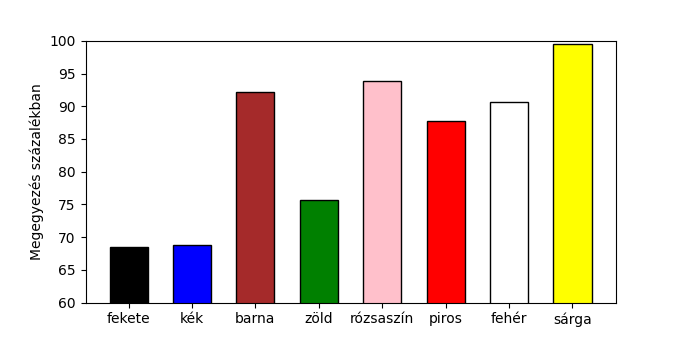
\includegraphics[width=140mm, keepaspectratio]{figures/match_values.png}
    \caption{Egy sárga golyó kivágott képére elvégzett mintaillesztések eredményei.}
    \label{fig:mintaillesztes_eredmeny}
\end{figure}

\par Az ábrán látható, hogy a mintaillesztés nehezen különbözteti meg az egyes színeket, szinte minden színhez 65\% -nál nagyobb megegyezési értékeket ad. Ez jól szemlélteti, hogy miért nem kerül közvetlen felhasználásra az alkalmazásban, azomban a adatkészlet készítéséhez felhasználható.
\par A mintaillesztés az alkalmazásban a \ref{cod:template_match} kódrészlet formájában kerül felhasználásra.

\vspace{2mm}
\hspace{-10mm}
\begin{minipage}{\linewidth}
\begin{lstlisting}[language=C++, numbers=left, caption={A mintaillesztés menete.}, label={cod:template_match}]
if (hsvMode) {
    cv::Mat templateHSV;
    cv::cvtColor(templateBGR, templateHSV, cv::COLOR_BGR2HSV);
    cv::matchTemplate(cutImageHSV, templateHSV, result, cv::TM_CCORR_NORMED);
}
else {
    cv::matchTemplate(cutImageBGR, templateBGR, result, cv::TM_CCORR_NORMED);
}

double maxValue;
cv::minMaxLoc(result, NULL, &maxValue);
\end{lstlisting}
\end{minipage}

\par Itt a \lstinline{hsvMode} logikai változó megadja, hogy a mintaillesztést BGR vagy HSV színformátumban végezze el a kód. A HSV módban történő illesztésnél szimplán átkonvertálom a mintát HSV formátumra a már jól ismert \lstinline{cv::cvtColor} függvénnyel\cite{opencv_docs}, majd mind a két módban úgyanúgy végrehajtom a mintaillesztést a \lstinline{cv::matchTemplate} függvénnyel\cite{kaehler2016learning,opencv_docs}. A függvény a \ref{for:cross_correlation} egyenlet alapján számolja ki a minta egyezőségét egy adott pontban. Paraméterként meg kell adni neki a képet amelyre a mintát szeretnénk illeszteni (\lstinline{cutImageBGR} vagy \lstinline{cutImageHSV}), a mintát (\lstinline{templateHSV} vagy \lstinline{templateBGR}), a kimeneti változónkat, amely ebben az esetben a \lstinline{result} mátrix, továbbá meg kell adnunk a mintaillesztés algorimust, ezt a \lstinline{cv::TM_CCORR_NORMED} konstans teszi meg.
\par A kapott mátrixból az egyezőséget reprezentáló értéket a \lstinline{cv::minMaxLoc} függvény\cite{opencv_docs} adja meg, ez a függvény kiszámolja, hogy a bemeneti mátrixon (\lstinline{result}) hol található és mennyi a minimum és maximum érték. Az egyezőség megállapításához ezesetben csak a maximum értékre van szükség, ezt a függvény harmadik paramétere adja meg \lstinline{maxValue} néven.
\par A fenti folyamat egy körre írja le a minta illesztését, ezt ciklusban az alkalmazás végrehajtja minden potenciális goylót leíró körre.

\subsection{Osztályozás neurális hálózattal}
A neurális hálózattal való osztályozás hasonlóan megy végbe, minta az előző alfejezetben megismert mintaillesztes. Az osztályozáshoz szükség van egy betanított neurális hálózatra, amit be kell tölteni az alkalmazásba, majd továbbítani neki a kör kivágott képét. A kivágott képet átadás előtt viszont módosítani kell, mégpedig úgy, hogy megegyezzen a neurális háló kívánt bemenetével.
\par Az általam használt modell bemenete egy olyan képet vár, amelynek hat intenzitásértéke van, azonban egy átlagos kivágott kép csupán három ilyen értékkel rendelkezik, ezek a BGR által reprezentált kék (blue), zöld (green) és piros (red) intenzitások, a másik három szükséges intenzitást a kép HSV értékei adják meg, ezek az árnyalat (hue), telítettség (saturation) és érték (value).
\par A kép intenzitásait összefűzve, majd azt továbbítva a hálózatnak, a kapott érték egy normalizált értékek listája, ami megadja, hogy egyes színek mennyire jellemzik a bemeneti képet. A \ref{fig:mintaillesztes_eredmeny} ábrához hasonlóan látható egy sárga golyó neurális hálózatos osztályozásának eredménye a \ref{fig:neuralis_osztalyozas_eredmeny} ábrán. Az ábrán látható, hogy míg a sárga érték nem mutatható teljesen az ábra intervallumán, hisz megegyezése közel 100\% -os (99,46\%), addig a többi színhez tartozó megegyezési értékek 0.1\% alá esnek. Ez is mutatja, hogy a módszer rendkívül pontosan meg tudja jósolni egy potenciálisan felismert golyó színét.

\begin{figure}[!ht]
    \centering
    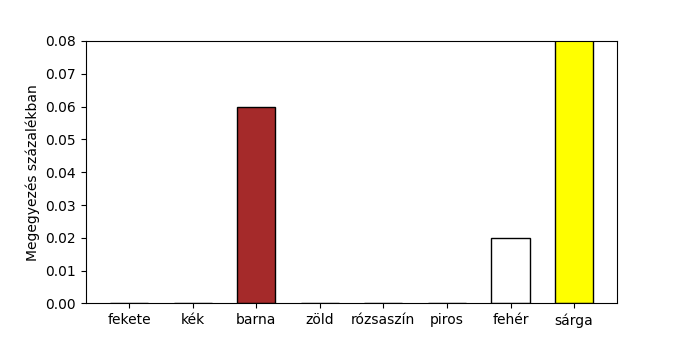
\includegraphics[width=140mm, keepaspectratio]{figures/neural_values.png}
    \caption{Egy sárga golyó kivágott képén neurális hálózattal történt becslés eredményei.}
    \label{fig:neuralis_osztalyozas_eredmeny}
\end{figure}

\par A felismerés végrehajtásához használt kód a \ref{cod:neural_predict} kódrészletben látható.

\vspace{2mm}
\hspace{-10mm}
\begin{minipage}{\linewidth}
\begin{lstlisting}[language=C++, numbers=left, caption={A neurális hálóval történő osztályozás menete.}, label={cod:neural_predict}]
std::vector<cv::Mat> channels = {cutImageBGR, cutImageHSV};
cv::Mat mixed;
cv::merge(channels, mixed);

fdeep::tensor input = fdeep::tensor_from_bytes(
    mixed.ptr(),
    static_cast<std::size_t>(mixed.rows),
    static_cast<std::size_t>(mixed.cols),
    static_cast<std::size_t>(mixed.channels()),
    0.0f,
    1.0f
);

std::vector<float> result = model.predict(input).to_vector();
\end{lstlisting}
\end{minipage}

\par A \ref{cod:neural_predict} kódrészletben elsősorban a kép intenzitás érékeit fűzzük össze, ezt a \lstinline{cv::merge} függvény\cite{opencv_docs} teszi meg, ami bemenetként kéri a két képet (BGR és HSV) egy tömb formájában, a kimenetet pedig a \lstinline{mixed} változóba teszi bele.
\par A hat színcsatornával rendelkező \lstinline{mixed} mátrixot ezekután egy ún. tensor típusra kell átalakítani, amelyet a neurális hálózat közvetlenül kezelni tud. Az átalakításhoz a \lstinline{fdeep::tensor_from_bytes} függvény\cite{frugally_deep2016} szükséges, amelynek paraméterként át kell adni a mátrixunk memóriacímének mutatóját (\lstinline{mixed.ptr()}), ez alapján tudja megállapítani a függvény az adatok helyzetét a memóriában, továbbá még át kell adni a mátrix szélességét (\lstinline{mixed.cols}), magasságát (\lstinline{mixed.rows}) és a színcsatornák számát (\lstinline{mixed.channels}). Az utolsó két paraméter megadja, hogy az intenzitás értékek 0 és 1 értékek közé legyenek skálázva. Ez egy 0 és 255 értékek között mozgó intenzitásnál, például 130, $\frac{130}{255} \approx 0.51$ értéket jelent.
\par A tensor-ra alakítás után a \lstinline{model.predict} függvénnyel\cite{frugally_deep2016} lehet a hálózat jóslását elvégezni, amely kimenete a \lstinline{result} változóba kerül. A kimenet egy lebegőpontos értékek tömbje lesz, ennek elemei adják meg, hogy egyes színek mennyire jellemzik az osztályozott képet. A legnagyobb tömb elemhez tartozó index jelöli a jósolt színt, hasonlóan az előző \ref{subsection:mintaillesztes_osztalyozas} alfejezetben megismert mintaillesztéshez.

\section{Játékmenet vizsgálati szempontok kiszámolása}